\documentclass[conference]{IEEEtran}
\usepackage{iftex}
\ifXeTeX
  \usepackage{fontspec}\setmainfont{texgyretermes}[Extension=.otf,UprightFont=*-regular,BoldFont=*-bold,ItalicFont=*-italic,BoldItalicFont=*-bolditalic] % Times + hrvatski znakovi (XeLaTeX/tectonic)
\else
  \usepackage[T1]{fontenc}\usepackage[utf8]{inputenc}\usepackage{newtxtext} % pdfLaTeX (npr. Overleaf)
\fi
\usepackage[croatian]{babel}
\usepackage{graphicx}
\usepackage{booktabs}
\usepackage{amsmath}
\usepackage{cite}
\usepackage{url}
\usepackage[hidelinks]{hyperref}
\graphicspath{{../retinal-vessel-segmentation/results/figures/}}

\begin{document}

\title{Segmentacija krvnih žila primjenom konvolucijskih neuronskih mreža\\
\large Izvještaj 1: analiza podataka i pregled literature}

\author{\IEEEauthorblockN{Tim 07: Erna Topalović, Lucija Bralić, Maja Ivandić, Sandro Kreštić}
\IEEEauthorblockA{Fakultet elektrotehnike i računarstva, Sveučilište u Zagrebu\\
Neuronske mreže, ak. god. 2026./2027.}}

\maketitle

\begin{abstract}
Cilj projekta je automatska segmentacija krvnih žila na medicinskim slikama pomoću konvolucijskih neuronskih mreža te ispitivanje utjecaja predobrade slike i arhitekture modela. Početno se usredotočujemo na fotografije očne pozadine. U ovoj fazi detaljno smo analizirali skupove FIVES (800 slika, $2048\times2048$) i CHASE\_DB1 (28 slika, $999\times960$). Analiza je otkrila nekoliko problema važnih za daljnji rad: dvije FIVES slike imaju potpuno prazne maske, na slikama loše kvalitete anotirane su samo vidljive žile, a 22 para slika prikazuju isto oko (gotovo identične maske), od čega pet parova prelazi službenu FIVES podjelu na skup za treniranje i testiranje. Takve slike grupirali smo pri podjeli kako ne bi došlo do curenja podataka. Pokazali smo i da zeleni kanal ima daleko najveći kontrast žila, da piksele žila čini samo oko 10\,\% vidnog polja te da je relativna širina žila jednaka u oba skupa, iako se rezolucije razlikuju 2,2 puta.
\end{abstract}

\section{Uvod}
Krvne žile mrežnice jedine su krvne žile koje se mogu neinvazivno promatrati, a promjene u njihovu obliku, širini i grananju povezane su s dijabetičkom retinopatijom, glaukomom, hipertenzijom i drugim bolestima~\cite{fraz2012survey}. Ručno označavanje žila na jednoj slici visoke rezolucije traje satima, pa je automatska segmentacija korisna kao prvi korak računalno potpomognute dijagnostike.

Segmentacija je ovdje binarna klasifikacija svakog piksela (žila ili pozadina). Zadatak je težak jer su žile tanke (često samo nekoliko piksela), slabog kontrasta, a slike se razlikuju po osvjetljenju, oštrini i patološkim promjenama koje mogu izgledati slično žilama.

Početno se usredotočujemo na fotografije očne pozadine, za koje postoje veliki javni skupovi s pikselnim anotacijama. Ako se pokaže da je taj zadatak nedovoljno zahtjevan, razmotrit ćemo proširenje na krvne žile iz drugih dijelova tijela. Kroz projekt planiramo tri eksperimentalne cjeline: (1) osnovni U-Net~\cite{ronneberger2015} na izvornim RGB slikama, (2) usporedbu predobrade (zeleni kanal, CLAHE, CLAHE + gamma korekcija) i (3) U-Net s predtreniranim koderom ResNet-34~\cite{he2016}. Ovaj izvještaj obuhvaća pregled literature (odjeljak~\ref{sec:lit}) i analizu podataka (odjeljak~\ref{sec:data}), a na kraju daje okvirni plan eksperimenata koji proizlazi iz analize (odjeljak~\ref{sec:plan}).

\section{Relevantna literatura}
\label{sec:lit}

\textbf{Skupovi podataka.} Klasični javni skupovi za segmentaciju žila mrežnice su DRIVE~\cite{staal2004} (40 slika, $565\times584$), STARE~\cite{hoover2000} (20 slika) i CHASE\_DB1~\cite{fraz2012ens} (28 slika $999\times960$, 14 djece, oba oka). Zbog malog broja slika rezultati na njima jako ovise o podjeli i lako se precijene. FIVES~\cite{jin2022fives} donosi 800 slika rezolucije $2048\times2048$ s pikselnim anotacijama, ravnomjerno podijeljenih na četiri kategorije (normalno, AMD, dijabetička retinopatija, glaukom), te uz svaku sliku ocjenu kvalitete (osvjetljenje/boja, zamućenje, nizak kontrast). Autori predlažu podjelu 600/200 koja uvažava te ocjene. Za CHASE\_DB1 postoje dvije neovisne ručne anotacije; slaganje dvaju anotatora (Dice $\approx0{,}78$) gruba je gornja granica koju model realno može doseći~\cite{fraz2012ens}.

\textbf{Klasične metode.} Pregledni radovi~\cite{fraz2012survey,moccia2018} dijele nenadzirane pristupe na filtriranje usklađenim filtrima, analizu Hessiana (\emph{vesselness}), praćenje žila i morfološke operacije, a nadzirane na klasifikaciju piksela iz ručno izrađenih značajki. Gotovo svi rade na \textbf{zelenom kanalu}, koji ima najveći kontrast između žila i pozadine, uz lokalno izjednačavanje histograma (CLAHE~\cite{zuiderveld1994}). Te dvije predobrade ispitujemo u eksperimentu~2.

\textbf{Duboko učenje.} Liskowski i Krawiec~\cite{liskowski2016} pokazali su da konvolucijska mreža koja klasificira patcheve nadmašuje klasične metode. U-Net~\cite{ronneberger2015} (koder--dekoder s preskočnim vezama) postao je standardna arhitektura za biomedicinsku segmentaciju jer dobro radi s malo slika i čuva fine detalje kroz preskočne veze. Galdran i sur.~\cite{galdran2022} pokazuju da vrlo mali, pažljivo treniran U-Net postiže gotovo iste rezultate kao znatno složeniji modeli, ali i da uspješnost znatno pada kad se testira na skupu drukčijem od onog za treniranje (\emph{cross-dataset}). To nam je važno jer kombiniramo dva izvora s različitim kamerama i rezolucijama. Kao jaču varijantu koristit ćemo U-Net s koderom ResNet-34~\cite{he2016} predtreniranim na ImageNetu, što je u praksi čest i jednostavan način za bolje značajke uz malo podataka.

\textbf{Funkcije gubitka i evaluacija.} Žile zauzimaju samo mali dio slike, pa se uz binarnu unakrsnu entropiju često koristi Dice gubitak~\cite{milletari2016}, koji je manje osjetljiv na neuravnoteženost klasa. clDice~\cite{shit2021} dodatno kažnjava prekide tankih žila i tako čuva povezanost (topologiju) mreže žila. Literatura~\cite{moccia2018,galdran2022} upozorava da točnost (\emph{accuracy}) na ovom zadatku malo govori jer je većina piksela pozadina. Zato kao glavnu metriku uzimamo Dice, uz preciznost, odziv, specifičnost i PR-AUC, i to računamo unutar vidnog polja.


\section{Analiza podataka}
\label{sec:data}
Sva analiza provedena je u Pythonu (NumPy, scikit-image, pandas). Kod je u bilježnici \texttt{01\_analiza\_podataka.ipynb} i modulima \texttt{prepare\_data.py} i \texttt{data\_analysis.py}. Sve brojke u ovom poglavlju dobivene su tim kodom.

\subsection{Namjena, izvor i veličina skupova}
\textbf{FIVES}~\cite{jin2022fives} sadrži 800 fotografija očne pozadine iz Second Affiliated Hospital of Zhejiang University (2016.--2021.), u formatu PNG $2048\times2048$ (RGB). U skupu je po 200 slika za svaku od četiri kategorije: normalno (N), senilna makularna degeneracija (AMD, A), dijabetička retinopatija (DR, D) i glaukom (G). Uz svaku sliku dana je binarna maska žila te tri binarne oznake kvalitete: problem s osvjetljenjem/bojom (IC), zamućenje (Blur) i nizak kontrast (LC). Autori nude podjelu 600/200 (train/test).

\textbf{CHASE\_DB1}~\cite{fraz2012ens} sadrži 28 slika ($999\times960$) oba oka 14 djece iz britanske studije CHASE, s maskama dvaju neovisnih anotatora. Kao referencu koristimo prvog anotatora, kao i literatura. Preuzeli smo verziju s HuggingFacea (\texttt{MedOtter/CHASE\_DB1}).

\textbf{Ulazi i oznake.} Ulaz je RGB slika, a oznaka binarna maska iste veličine (provjereno za sve slike; sve maske imaju točno dvije vrijednosti, 0 i 255). Deset FIVES maski spremljeno je kao RGBA umjesto RGB. Provjerili smo da je sadržaj isti u R, G i B kanalu, pa uvijek čitamo prvi kanal.

\begin{figure*}[t]
\centering
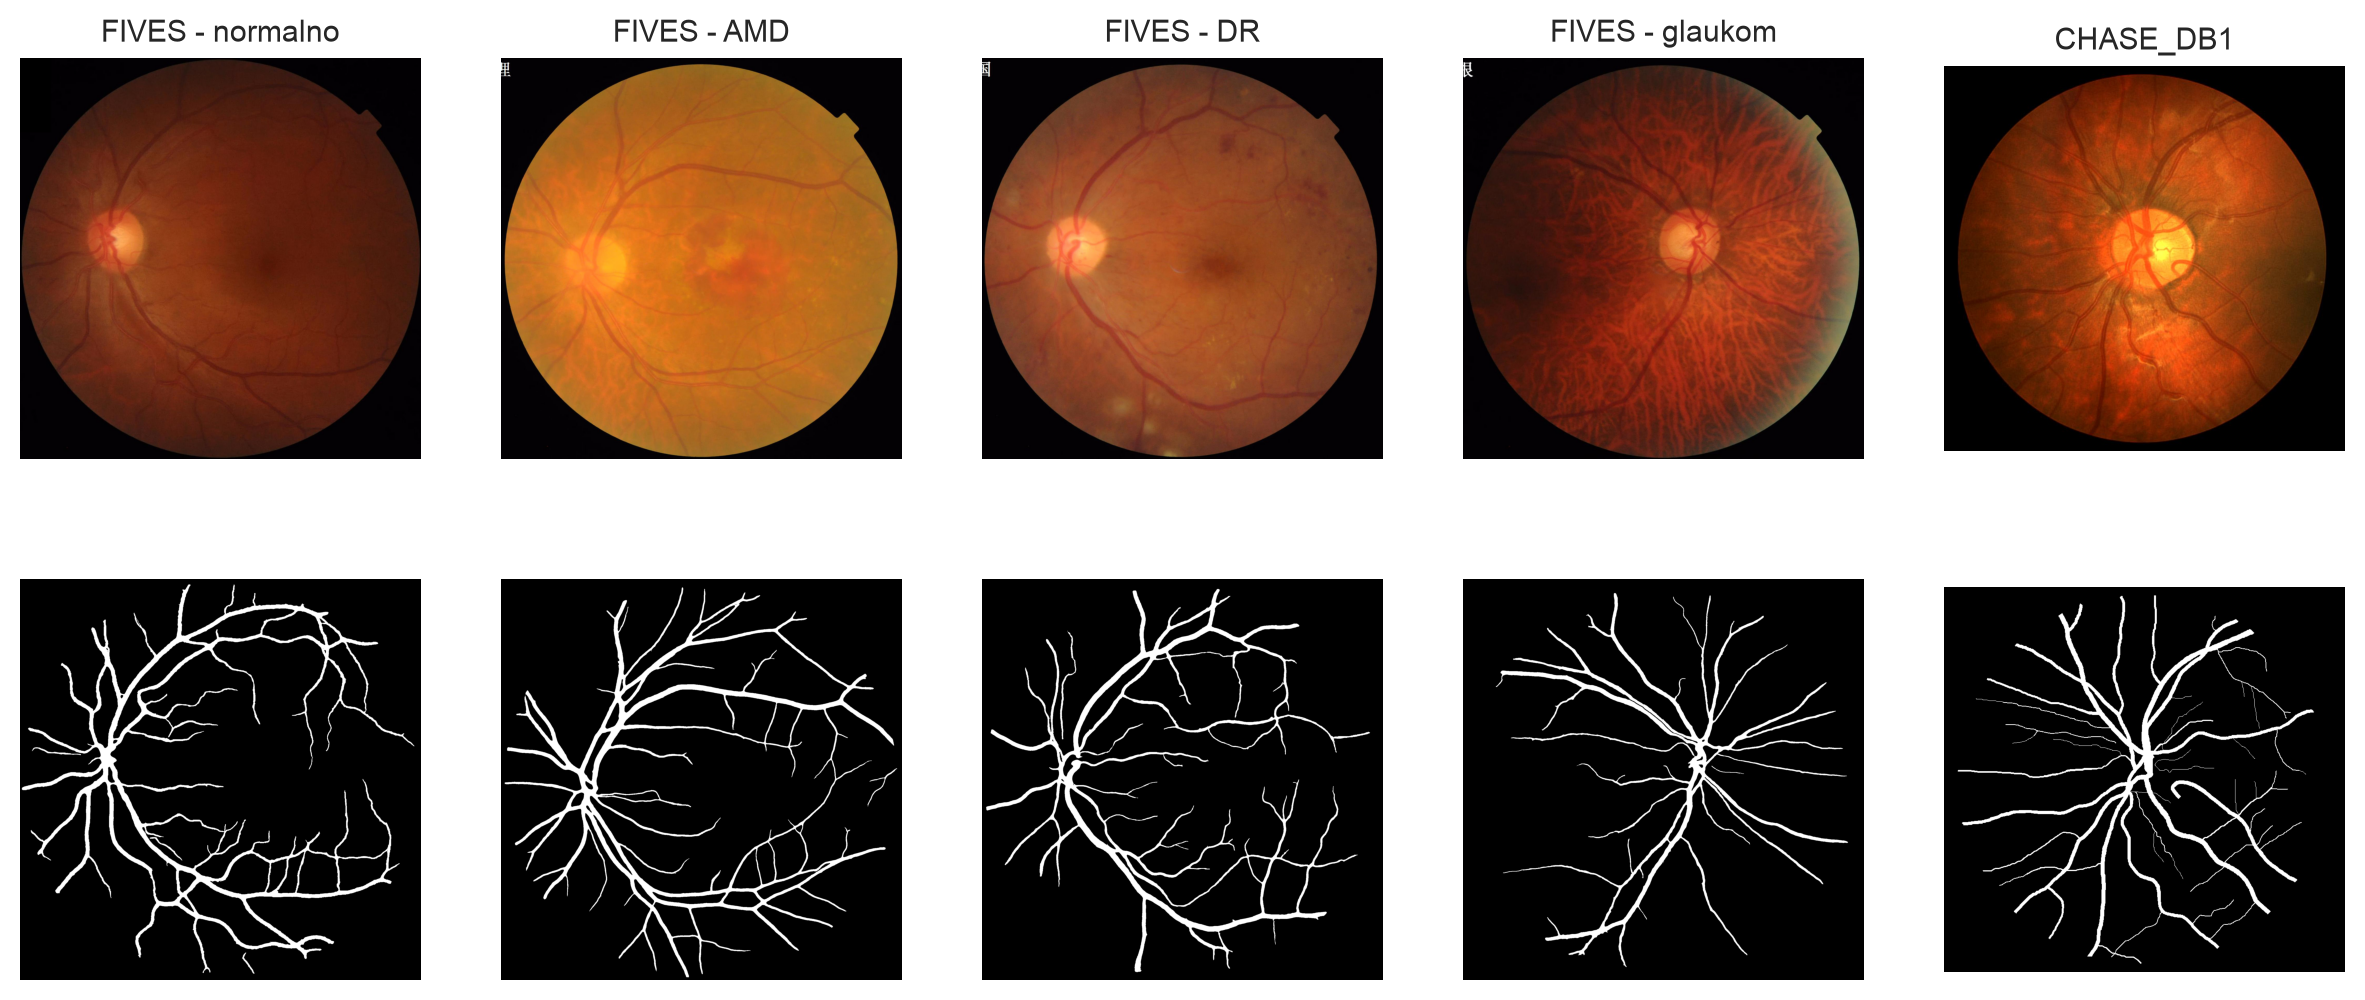
\includegraphics[width=0.9\textwidth]{fig_examples.png}
\caption{Primjeri slika (gore) i referentnih maski (dolje) za svaku kategoriju FIVES-a i za CHASE\_DB1. Kod glaukoma se u pozadini vide žile žilnice (koroide) koje nisu označene. U gornjem lijevom kutu FIVES slika vidi se sitan tekst.}
\label{fig:examples}
\end{figure*}

\subsection{Podjela na skupove za treniranje, validaciju i testiranje}
\label{sec:split}
Prema projektnom planu oba skupa spajamo i dijelimo na približno 70/15/15\,\%. Podjela je \textbf{stratificirana} po paru (skup, kategorija bolesti), tako da su oba izvora i sve bolesti jednako zastupljeni u svakom podskupu. Provodi se po \textbf{grupama}, a ne po pojedinim slikama:
\begin{itemize}
\item u CHASE\_DB1 grupa je dijete (oba oka zajedno), pa dobivamo 20/4/4 slike;
\item u FIVES-u nema identifikatora pacijenta, pa grupe gradimo iz sličnosti maski (odjeljak~\ref{sec:dups}).
\end{itemize}
Dvije slike s praznom maskom izbacili smo (odjeljak~\ref{sec:problems}). Konačna podjela ima \textbf{579 / 122 / 125} slika (tablica~\ref{tab:split}). Podjelu radimo na razini cijelih slika, prije izrezivanja patcheva, i spremamo je u \texttt{split.csv} (sjeme 42), tako da svi eksperimenti koriste istu podjelu. Prosječan udio žila u FOV-u gotovo je jednak u sva tri podskupa (9,6\,\%, 9,3\,\%, 9,5\,\%).

\begin{table}[t]
\centering
\caption{Konačna podjela podataka (broj slika)}
\label{tab:split}
\begin{tabular}{llrrrr}
\toprule
Skup & Kategorija & train & val & test & ukupno\\
\midrule
FIVES & normalno & 140 & 30 & 30 & 200\\
FIVES & AMD & 139 & 29 & 32 & 200\\
FIVES & DR & 140 & 30 & 30 & 200\\
FIVES & glaukom & 140 & 29 & 29 & 198\\
CHASE\_DB1 & normalno & 20 & 4 & 4 & 28\\
\midrule
\multicolumn{2}{l}{Ukupno} & 579 & 122 & 125 & 826\\
\bottomrule
\end{tabular}
\end{table}

\subsection{Osnovna statistika}
Za svaku sliku izračunali smo niz značajki (tablica~\ref{tab:stats}). \emph{Vidno polje} (FOV) je kružno područje fotografije, dobiveno pragom ($>4$) na najsvjetlijem kanalu, uz zadržavanje najveće komponente. \emph{Širinu žile} računamo na skeletu maske kao dvostruku udaljenost do ruba maske. \emph{Lokalni kontrast} je Weberov kontrast u zelenom kanalu između piksela žile i prstena pozadine širine 1\,\% promjera FOV-a oko žila: $C=(\bar{I}_{\text{okolina}}-\bar{I}_{\text{žila}})/\bar{I}_{\text{okolina}}$. \emph{Oštrinu} mjerimo kao varijancu Laplaceova operatora na zelenom kanalu smanjenom na $1024\times1024$.

\begin{table*}[t]
\centering
\caption{Statistike po slici: prosjek (medijan) [min, max]}
\label{tab:stats}
\begin{tabular}{lcc}
\toprule
Značajka & FIVES ($n=798$) & CHASE\_DB1 ($n=28$)\\
\midrule
Udio žila u FOV [\%] & 9,6 (10,2) [0,9; 14,5] & 10,0 (10,4) [7,2; 12,2]\\
Promjer FOV [px] & 2033 & 921\\
Sr. širina žile [px] & 13,2 (13,3) [8,5; 19,8] & 6,1 (6,0) [4,9; 7,3]\\
Sr. širina / promjer FOV [\textperthousand] & 6,5 & 6,6\\
Udio tankih žila [\%] & 28,4 (28,1) [7,7; 52,8] & 30,2 (30,5) [13,2; 44,5]\\
Lokalni kontrast (G) & 0,12 (0,12) [$-$0,07; 0,28] & 0,14 (0,14) [0,05; 0,18]\\
Oštrina & 13,6 (12,6) [1,1; 40,3] & 11,7 (11,2) [7,8; 17,6]\\
Br. povezanih komponenti & 4,6 (4) [1; 41] & 2,9 (2) [1; 11]\\
\bottomrule
\end{tabular}
\end{table*}

Glavna opažanja:
\begin{itemize}
\item \textbf{Neuravnoteženost klasa.} Žile čine prosječno 9,6\,\% piksela unutar FOV-a, odnosno omjer pozadine i žila na cijeloj slici iznosi oko 12,6\,:\,1. Model koji sve proglasi pozadinom imao bi točnost oko 92\,\%, pa točnost nije prikladna metrika. Koristimo Dice i PR-AUC, a za gubitak kombinaciju BCE i Dice~\cite{milletari2016}.
\item \textbf{Rezolucija.} U pikselima su FIVES žile dvostruko šire (13,2 naspram 6,1~px), ali je relativno prema promjeru FOV-a širina gotovo jednaka (6,5 naspram 6,6\,\textperthousand). Razlika je, dakle, samo u rezoluciji slike. Zato ćemo CHASE slike prije treniranja skalirati tako da FOV ima isti promjer kao u FIVES-u (faktor $\approx2{,}2$). Inače bi patch $768\times768$ obuhvaćao vrlo različit dio mrežnice.
\item \textbf{Tanke žile.} Kao tanke definiramo točke skeleta širine manje od 4\,\textperthousand\ promjera FOV-a ($\approx$8~px na FIVES-u, $\approx$3,7~px na CHASE-u). Takvih je oko 28--30\,\% ukupne duljine žila (slika~\ref{fig:width}). Tanke žile zauzimaju malo piksela, pa ih Dice slabo "kažnjava", iako su klinički važne. Zato ćemo ih posebno analizirati u rezultatima.
\item \textbf{Povezanost.} Maske su uglavnom povezane: medijan je 4 komponente, a udio piksela u komponentama manjim od 50~px zanemariv je ($<0{,}001$\,\%). Prekidi u predviđenim maskama bit će, dakle, pogreška modela, a ne svojstvo anotacija.
\end{itemize}

\begin{figure}[t]
\centering
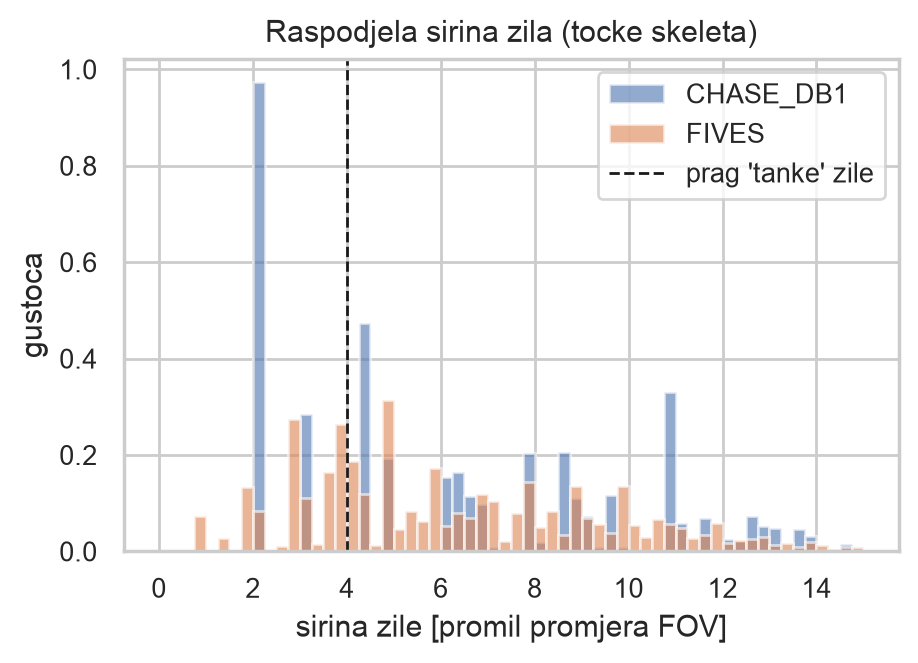
\includegraphics[width=\columnwidth]{fig_width_hist.png}
\caption{Raspodjela širina žila (točke skeleta) relativno prema promjeru FOV-a. Isprekidana linija je prag za tanke žile.}
\label{fig:width}
\end{figure}

\subsection{Raspodjela kategorija i kvalitete}
Kategorije u FIVES-u potpuno su uravnotežene (po 200), ali kvaliteta slika među njima nije (slika~\ref{fig:dist}, desno). Bar jedan problem kvalitete ima 25,8\,\% FIVES slika. Kod glaukoma 46\,\% slika ima problem s osvjetljenjem, 29\,\% zamućenje, a 16\,\% nizak kontrast. Kod normalnih slika zamućenje se gotovo ne pojavljuje (1,5\,\%). \emph{Bolest i kvaliteta slike su, dakle, povezane}: lošiji rezultat na glaukomu ne mora značiti da je bolest sama po sebi teža za segmentaciju, nego može biti posljedica lošijih slika. To ćemo uzeti u obzir pri analizi pogrešaka (rezultate ćemo prikazati i po kategoriji i po kvaliteti).

\begin{figure}[t]
\centering
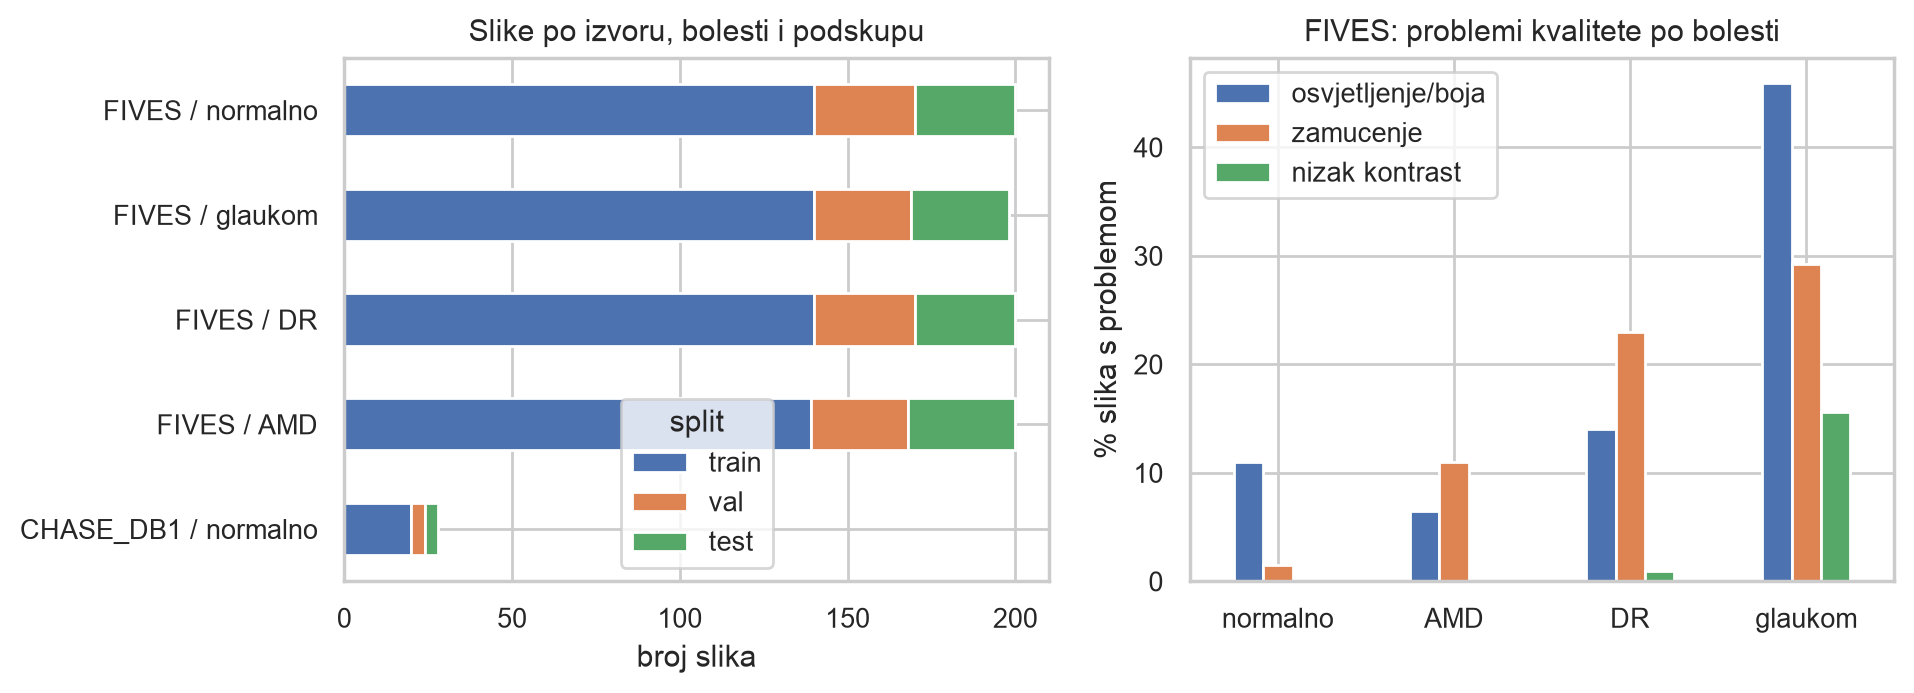
\includegraphics[width=\columnwidth]{fig_distribution.png}
\caption{Lijevo: broj slika po izvoru, kategoriji i podskupu. Desno: udio FIVES slika s problemom kvalitete po kategoriji.}
\label{fig:dist}
\end{figure}

Udio žila po kategorijama (slika~\ref{fig:vessel}) najveći je kod normalnih slika (11,3\,\%), a najmanji i najraspršeniji kod glaukoma (8,5\,\%). Djelomično je to stvarni učinak bolesti (stanjivanje žila), a djelomično posljedica anotacija na lošim slikama (sljedeći odjeljak).

\begin{figure*}[t]
\centering
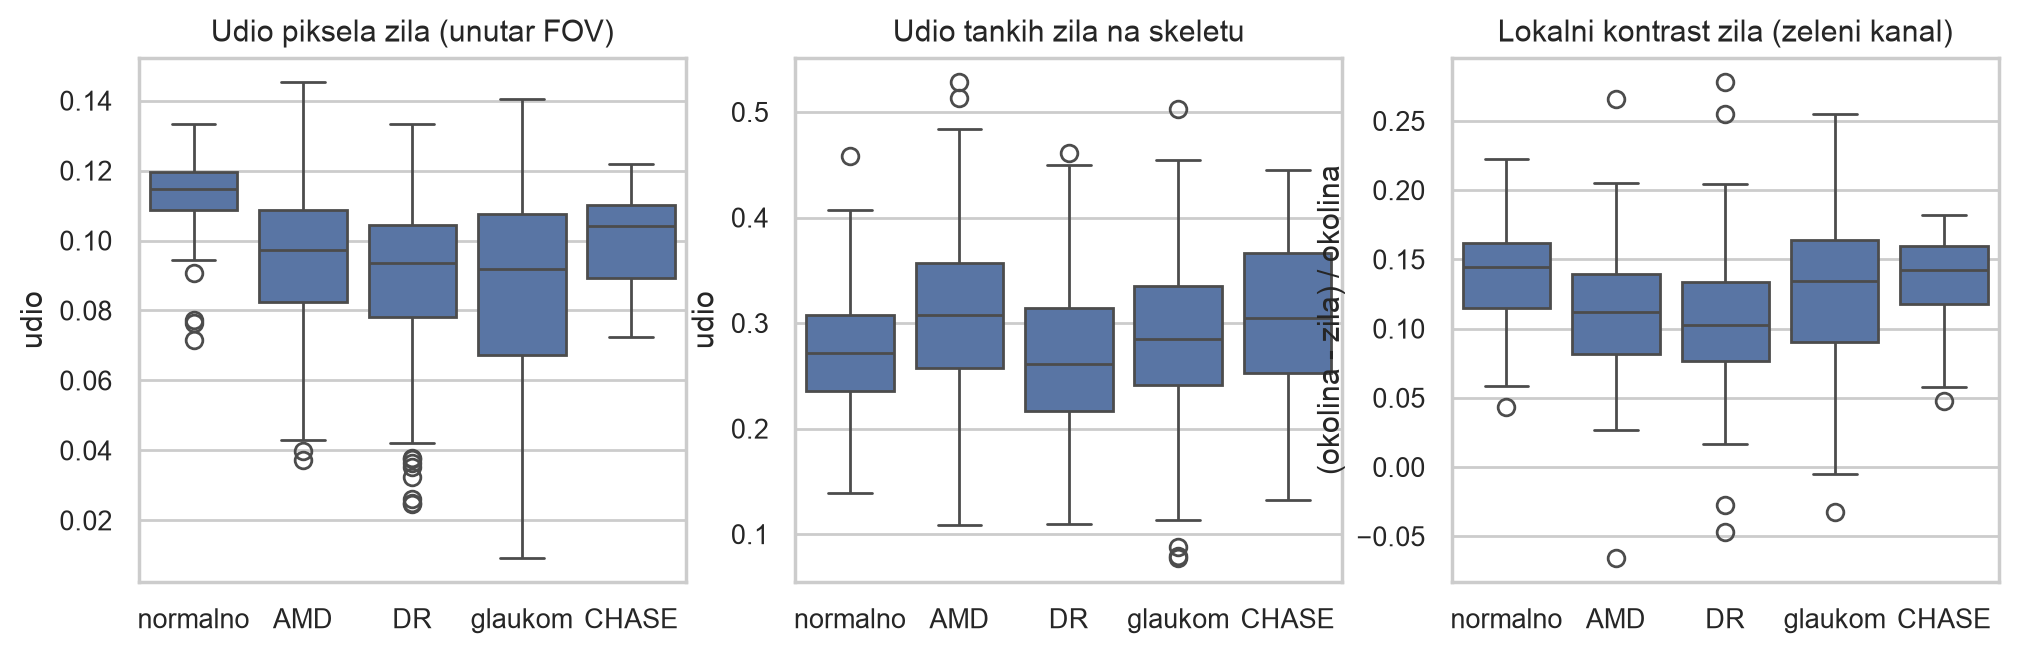
\includegraphics[width=0.85\textwidth]{fig_vessel_stats.png}
\caption{Udio piksela žila u FOV-u, udio tankih žila i lokalni kontrast žila po kategoriji.}
\label{fig:vessel}
\end{figure*}

\subsection{Kanali boje i predobrada}
Lokalni kontrast žila izračunali smo zasebno za R, G i B kanal na 80 slučajno odabranih slika iz skupa za treniranje (slika~\ref{fig:channel}). Zeleni kanal ima medijan kontrasta 0,12, plavi 0,04, a crveni samo 0,01: crveni kanal je često zasićen, a plavi taman i šumovit. To je u skladu s literaturom~\cite{fraz2012survey} i motivira eksperiment~2. Slika~\ref{fig:prep} prikazuje varijante predobrade koje ćemo usporediti. CLAHE~\cite{zuiderveld1994} vidljivo pojačava tanke žile, ali i šum pozadine. Hoće li to pomoći ili odmoći mreži, provjerit ćemo eksperimentom.

\begin{figure}[t]
\centering
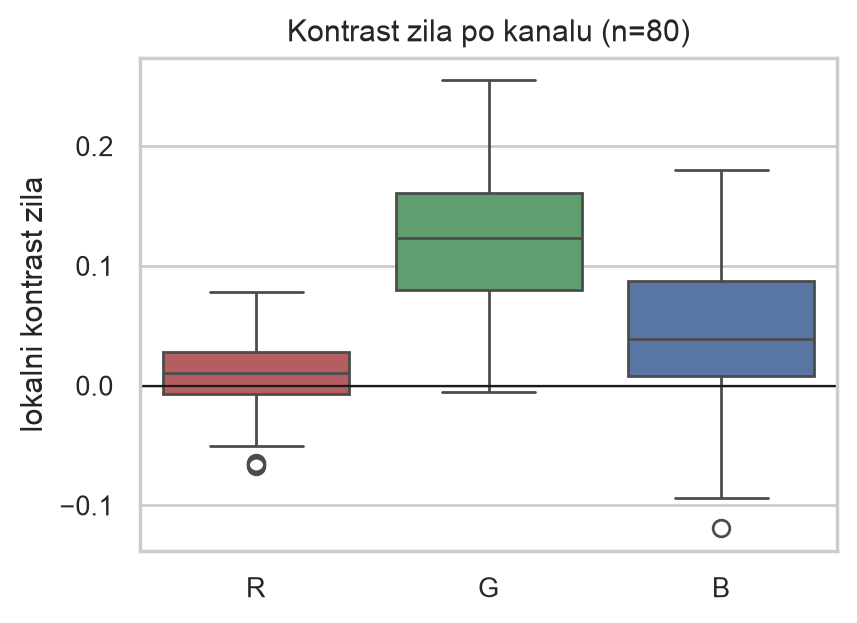
\includegraphics[width=0.75\columnwidth]{fig_channel_contrast.png}
\caption{Lokalni (Weberov) kontrast žila u R, G i B kanalu (80 slika iz skupa za treniranje).}
\label{fig:channel}
\end{figure}

\begin{figure}[t]
\centering
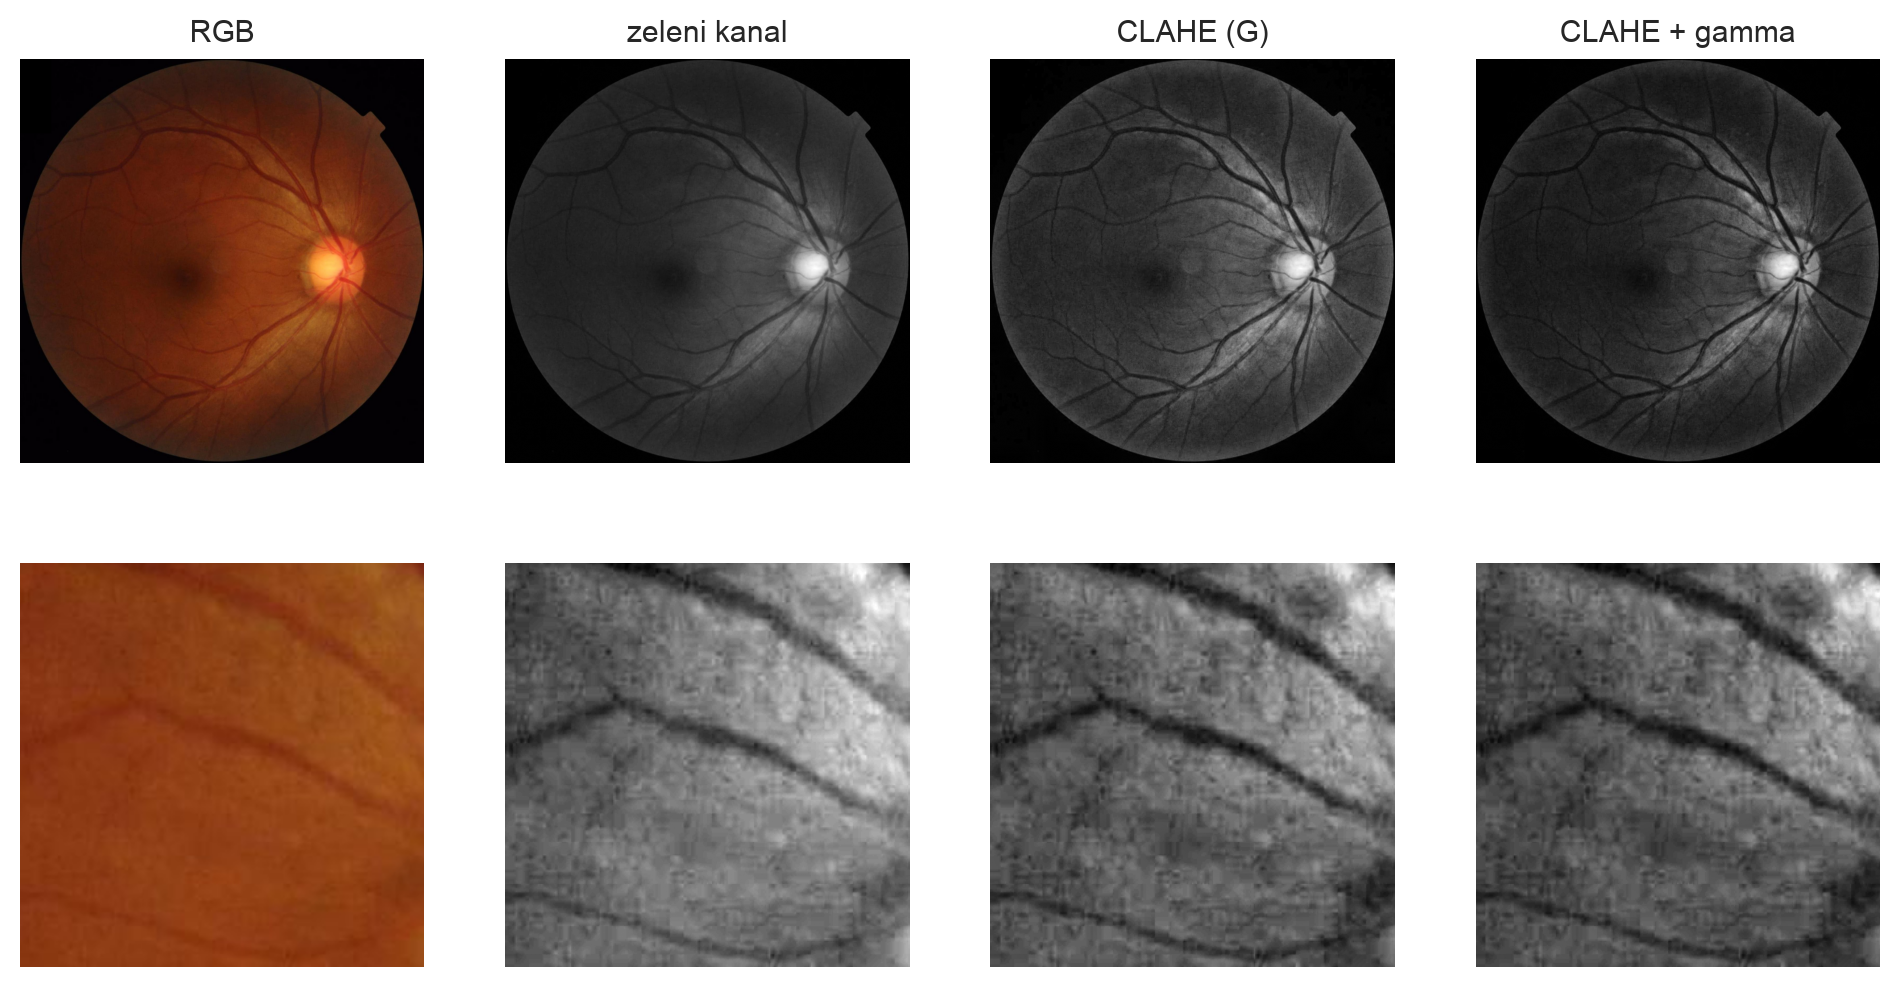
\includegraphics[width=\columnwidth]{fig_preprocessing.png}
\caption{Varijante predobrade iz eksperimenta 2 na slici FIVES train 455\_N (gore) i uvećani isječak s tankim žilama (dolje).}
\label{fig:prep}
\end{figure}

\subsection{Odnosi između značajki}
Slika~\ref{fig:corr} prikazuje Spearmanovu korelaciju značajki na FIVES-u. Najvažniji odnosi:
\begin{itemize}
\item oznaka \emph{Blur ok} pozitivno korelira s udjelom žila ($\rho=0{,}55$) i lokalnim kontrastom ($\rho=0{,}44$). Na zamućenim slikama prosječno je označeno samo 6,1\,\% piksela kao žila, naspram 10,6\,\% na oštrim;
\item naša mjera oštrine (varijanca Laplacea) gotovo je jednaka srednjoj svjetlini zelenog kanala ($\rho=0{,}89$), pa ne mjeri pouzdano zamućenje. Za kvalitetu ćemo zato koristiti oznake iz FIVES-a;
\item udio tankih žila i srednja širina snažno su negativno povezani ($\rho=-0{,}83$), što je očekivano i potvrđuje da je mjera širine smislena.
\end{itemize}

\begin{figure}[t]
\centering
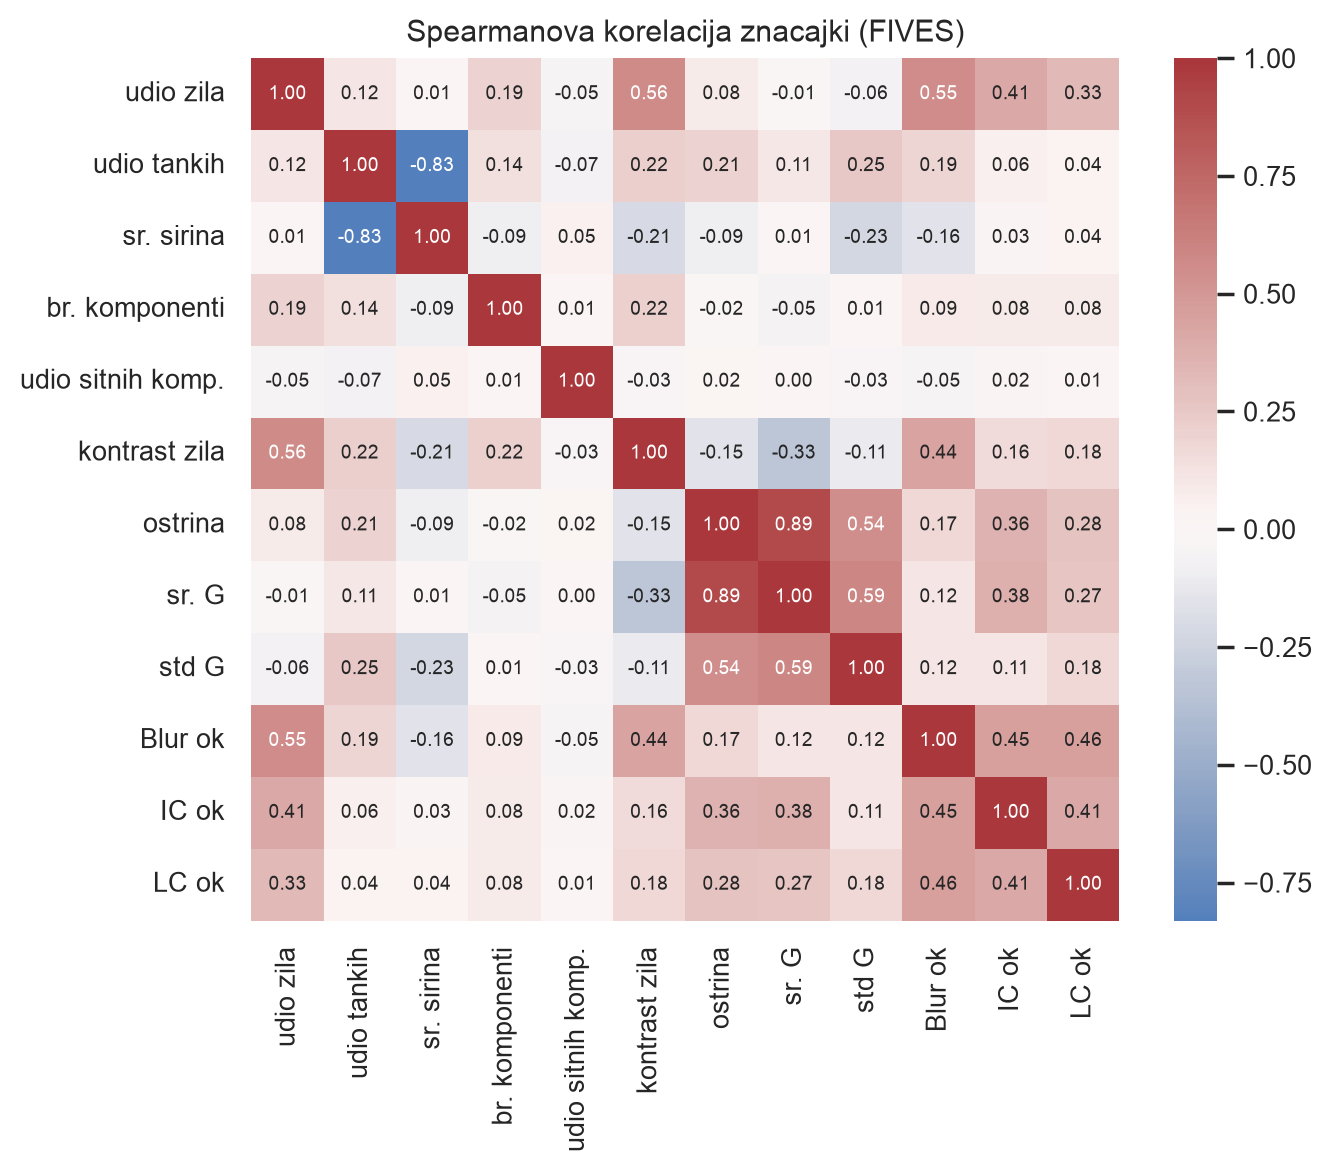
\includegraphics[width=\columnwidth]{fig_correlation.png}
\caption{Spearmanova korelacija značajki slika i oznaka kvalitete (FIVES).}
\label{fig:corr}
\end{figure}

\subsection{Potencijalni problemi u podacima}
\label{sec:problems}
\textbf{Prazne maske.} Slike FIVES train 447\_G i 448\_G gotovo su potpuno crne, a njihove maske ne sadrže nijedan piksel žile. Takva oznaka bila bi za model pogrešna (žile postoje, samo nisu vidljive), pa smo te dvije slike izbacili.

\textbf{Djelomične anotacije.} Najmanji udio žila (0,9--2,5\,\%) imaju mutne i tamne slike, uglavnom glaukom (npr. train 316\_G, test 122\_G). Na njima su označene samo dobro vidljive veće žile. Ako model na takvoj slici pronađe žilu koju anotator nije označio, to će se računati kao lažno pozitivno. Te slike zadržavamo jer predstavljaju stvarne uvjete snimanja, ali ćemo pri evaluaciji posebno prikazati rezultate na slikama loše kvalitete.

\textbf{Neoznačene žile žilnice.} Kod dijela slika glaukoma (tzv. tigroidna očna pozadina, slika~\ref{fig:examples}) vide se krupne žile žilnice koje nisu dio maske. Očekujemo da će ih model ponekad zamijeniti za žile mrežnice.

\textbf{Tekst u kutu.} Na 71,7\,\% FIVES slika u gornjem lijevom kutu, izvan FOV-a, nalazi se sitan znak (slika~\ref{fig:examples}). Budući da nije povezan s kategorijom ni maskom, ne očekujemo da će ga model koristiti kao prečac, ali ga pri evaluaciji isključujemo jer metrike računamo samo unutar FOV-a.

\textbf{Stršeće vrijednosti i nedostajući podaci.} Nema nedostajućih slika ni maski. Datoteka \texttt{Thumbs.db} u mapi FIVES train jedini je višak i ignoriramo je. Stršeće vrijednosti su gore opisane slike s malim udjelom žila i negativnim kontrastom (jako tamne slike), koje zadržavamo.

\subsection{Duplikati i curenje podataka}
\label{sec:dups}
FIVES ne navodi identifikator pacijenta, pa ne znamo potječu li dvije slike od istog oka. Takve smo slike pokušali pronaći usporedbom smanjenih maski ($64\times64$) za svaki par od 826 slika, mjereći IoU. Za nesrodne mrežnice IoU je nizak: medijan 0,20, a 99,99. percentil 0,36. Pronašli smo \textbf{22 para s IoU $>0{,}5$} (slika~\ref{fig:dups}):
\begin{itemize}
\item 8 parova s IoU $>0{,}9$ praktički su ista snimka istog oka (npr. test 022\_A i 023\_A imaju identične maske);
\item 7 parova (IoU $\approx0{,}65$--$0{,}69$) prikazuje isto oko s \emph{različitim dijagnozama}: jedna slika označena je kao normalna, a druga kao glaukom;
\item \textbf{5 parova prelazi službenu FIVES podjelu} na train i test (npr. train 174\_D i test 054\_D, IoU 0,998). To je curenje podataka u službenoj podjeli koje bi napuhalo rezultate na testnom skupu.
\end{itemize}
Sve takve slike spojili smo u iste grupe (\emph{union-find}), pa pri podjeli uvijek završe u istom podskupu. Nakon podjele nijedan par nije razdvojen. Napominjemo da ovom metodom ne možemo pronaći lijevo i desno oko istog pacijenta, pa određeno curenje na razini pacijenta i dalje može postojati.

\begin{figure}[t]
\centering
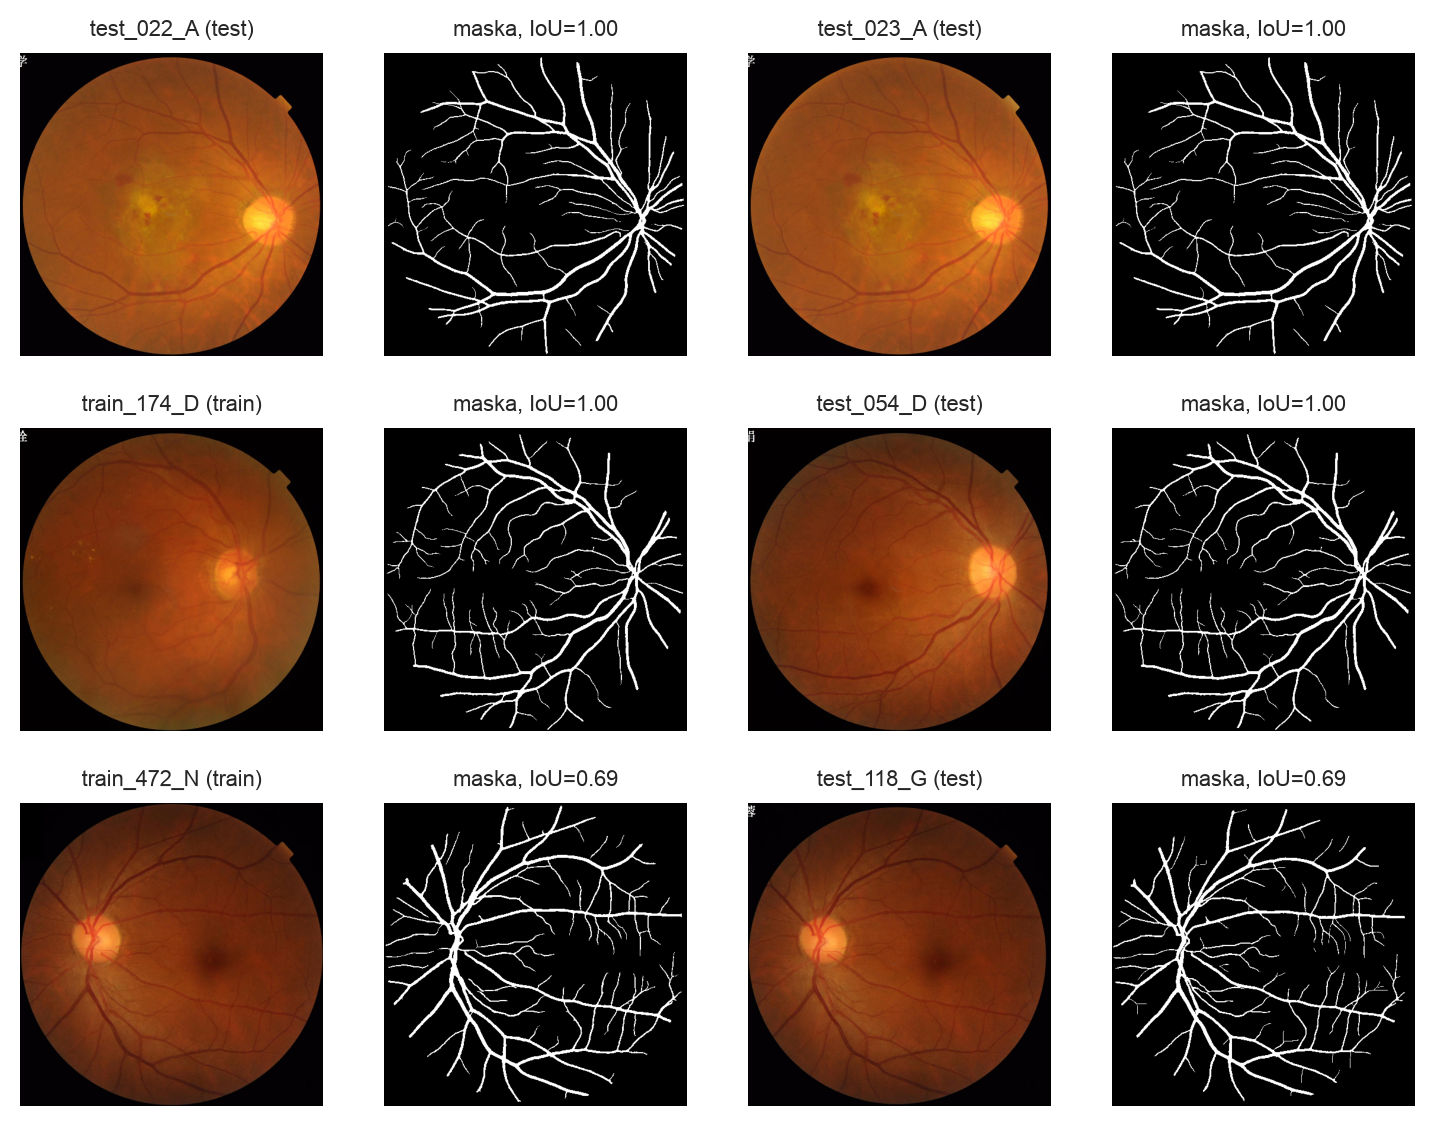
\includegraphics[width=\columnwidth]{fig_duplicates.png}
\caption{Primjeri parova istog oka u FIVES-u. Gore: identična snimka; sredina: par koji prelazi službeni train/test; dolje: isto oko s oznakama ``normalno'' i ``glaukom''.}
\label{fig:dups}
\end{figure}

\subsection{Patchevi}
Ako sliku $2048\times2048$ podijelimo na patcheve $768\times768$ bez preklapanja (3192 patcha), samo 0,7\,\% patcheva ne sadrži nijednu žilu, a 2,4\,\% ih ima manje od 1\,\% žila. Uzorkovanje patcheva zato neće proizvesti mnogo ``praznih'' primjera. Tri patcha po osi bez preklapanja ne pokrivaju cijelu sliku ($3\cdot768>2048$), pa ćemo za treniranje koristiti nasumične izreze, a za rekonstrukciju klizni prozor s preklapanjem.

\subsection{``Laki'' i ``teški'' primjeri}
Primjere smo rangirali po lokalnom kontrastu, oštrini i udjelu tankih žila (slika~\ref{fig:easyhard}). Lakima očekujemo oštre slike dobre kvalitete s jasnim kontrastom, uglavnom iz kategorije normalno. Teškima smatramo tamne i mutne slike (gotovo isključivo glaukom), na kojima je kontrast žila blizu nule i anotacija djelomična. Na njima očekujemo i najveće neslaganje modela s maskom. Dodatno, teškima smatramo slike s patologijama koje nalikuju žilama (krvarenja kod DR-a, žile žilnice kod glaukoma) i područje optičkog diska, gdje se žile gusto preklapaju.

\begin{figure}[t]
\centering
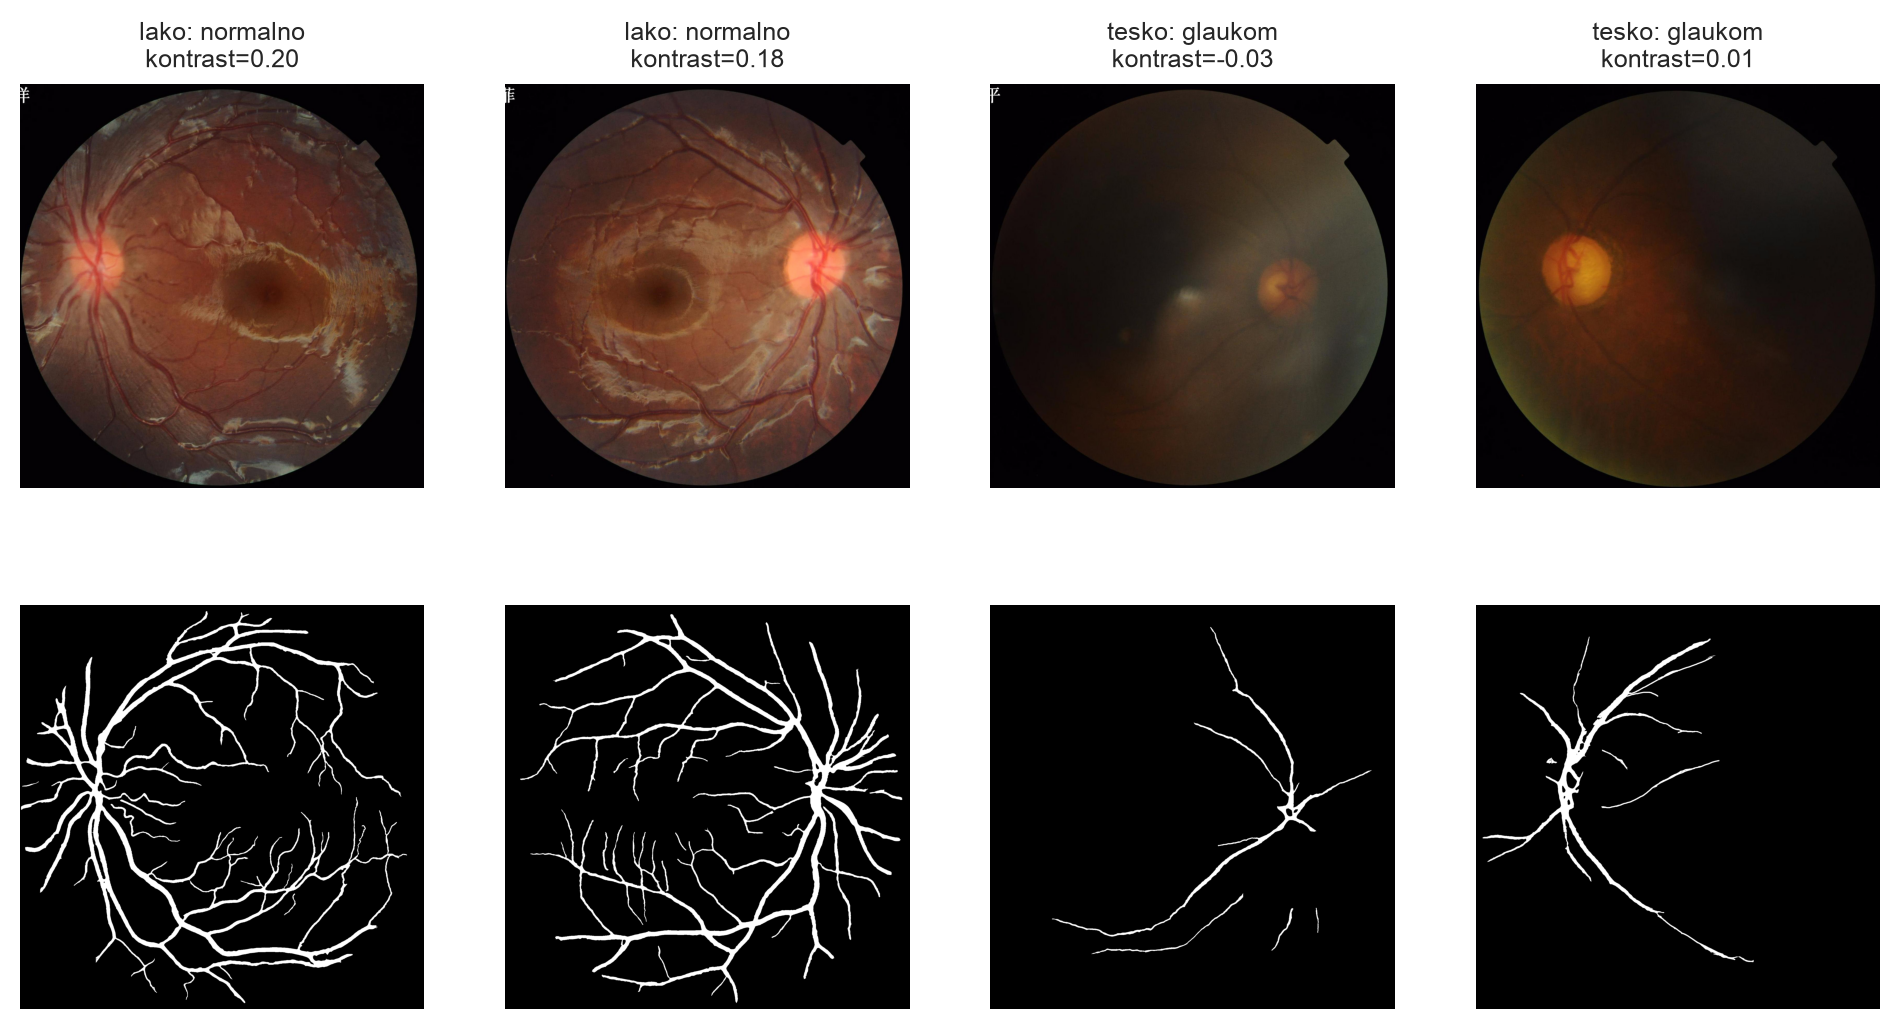
\includegraphics[width=\columnwidth]{fig_easy_hard.png}
\caption{Primjeri koje smatramo ``lakima'' (lijevo) i ``teškima'' (desno), uz lokalni kontrast u zelenom kanalu.}
\label{fig:easyhard}
\end{figure}

\section{Okvirni plan eksperimenata}
\label{sec:plan}
Na temelju analize zadržavamo tri eksperimenta iz projektnog plana, uz ove odluke:
\begin{enumerate}
\item \textbf{Ulaz:} CHASE slike skaliramo na promjer FOV-a FIVES-a. Treniramo na nasumičnim izrescima $768\times768$, a predviđanje radimo kliznim prozorom s preklapanjem, uz spajanje u cijelu sliku.
\item \textbf{Gubitak:} BCE + Dice zbog neuravnoteženosti klasa (omjer $\approx$\,12:1).
\item \textbf{Evaluacija:} Dice, preciznost, odziv, specifičnost i PR-AUC na cijelim testnim slikama, samo unutar FOV-a. Rezultate prikazujemo zasebno po izvoru (FIVES/CHASE), kategoriji bolesti i kvaliteti slike. Uz to računamo Dice samo na tankim žilama.
\item \textbf{E1:} U-Net na RGB slikama; \textbf{E2:} zeleni kanal, CLAHE, CLAHE + gamma; \textbf{E3:} U-Net s koderom ResNet-34 predtreniranim na ImageNetu, na najboljoj predobradi iz E2 (izbor na validacijskom skupu).
\end{enumerate}

\section{Zaključak}
Skup od 826 iskoristivih slika iz dva izvora dovoljan je za treniranje i usporedbu U-Net modela. Analiza je pokazala da je glavni izazov kvaliteta podataka, a ne njihova količina: neuravnoteženost klasa, tanke žile, djelomične anotacije na lošim slikama, povezanost bolesti i kvalitete te višestruke snimke istog oka koje uzrokuju curenje u službenoj podjeli FIVES-a. Te smo probleme uzeli u obzir u podjeli podataka i planu evaluacije.

\bibliographystyle{IEEEtran}
\bibliography{literatura}

\end{document}
